%%%%%%%%%%%%%%%%%%%%%%%%%%%%%%%%%%%%%%%%%%%%%%%%%%%%%%%%%%%%%%%%%%%%%%%%
% TFG: Vigilancia Tecnológica y Minería de Opiniones en RRSS
% Escuela Técnica Superior de Ingenierías Informática y de Telecomunicación
% Realizado por: Miguel Keane Cañizares
% Contacto: miguekeca@correo.ugr.es 
%%%%%%%%%%%%%%%%%%%%%%%%%%%%%%%%%%%%%%%%%%%%%%%%%%%%%%%%%%%%%%%%%%%%%%%%

\chapter{Diseño}


El diseño del proyecto tendrá como objetivo mantener la mayor simplicidad y efectividad posible. Para ello primeramente se diseñarán los diferentes requerimientos. 

\subsection{Requerimientos Funcionales}

\begin{itemize}
	\item Registro en la API de Twitter haciendo uso de las credenciales obtenidas.
	\item Introducción de palabras clave para la búsqueda en Twitter.
	\item Seleccionar idioma de los tweets que serán descargados.
	\item Realizar búsquedas de las palabras claves indicadas.
	\item Descargar un tweet y guardarlo en una variable.
	\item Parsear la variable que contenga el tweet en un tipo de dato JSON, más manejable.
	\item Descomposición del Tweet en diferentes variables que contengan la diferente información del mismo.
	\item Aceptar tweets de más de 140 caracteres con el modo \textit{extended\_tweet}.
	\item Creación de base de datos MongoDB con el nombre deseado.
	\item Conexión con la base de datos MongoDB.
	\item Inicialización de colección \textit{tweets} en la base de datos MongoDB.
	\item Almacenamiento de los datos parseados del tweet en un documento MongoDB. 
	
	\item Conexión con la API MeaningCloud con la contraseña proporcionada. 
	\item Introducción del nombre del fichero CSV. 
	\item Comprobación de si el fichero CSV existe con prioridad, de no ser así, crearlo con una primera fila con las caberas de los datos. 
	\item Recorrer la colección \textit{tweets}, enviando uno a uno el cuerpo del tweet a MeaningCloud para ser analizado. 
	\item Almacenamiento y gestión de la respuesta de MeaningCloud.
	\item Distinción entre los diferentes elementos en la respuesta de MeaningCloud. 
	\item Almacenamiento de los datos que se desean conservar del análisis en un fichero CSV y en una nueva colección MongoDB, llamada \textit{concepts}.
	
	\item Creación de nubes de palabras en formato png. 
	\item Creación de gráficas de barras con matplotlib para estudiar los resultados del análisis de sentimientos. 
	\item Introducción de imágenes modelo para la creación de nubes de palabra.
	
	
	
	


\end{itemize}


\subsection{Requerimientos No Funcionales}

\begin{itemize}

	\item Todos las conexiones con Twitter deben tener forma de manejar errores en caso de haberlos. Indicando por pantalla cual ha sido el error y, si es posible, evitar que el programa deje de ejecutarse por el mismo. 
	\item Los datos almacenados deben ser ampliables y reutilizables. 
	\item Evitar los tipos de datos Retweets, ya que estos solo proporcionan información repetida que no será de utilidad para su posterior análisis.
	\item Al almacenar datos en la base de datos, deben preveerse formas de manejar excepciones en caso de error. Priorizando que la ejecución del programa no sea interrumpida y que no haya pérdida de información. 
	
	\item Almacenar las contraseñas en un fichero aparte que será ignorado por Github, para evitar publicar información privada.
	
	\item Manejar posibles errores en la conexión a MeaningCloud, evitando que se interrumpa el proceso de análisis. 
	
	\item Manejar códigos de respuesta de MeaningCloud. Es posible que sin haber un error, el análisis no tenga éxito, se deben manejar estos casos para el programa no interrumpa su ejecución. 
	
	\item Evitar que las comas del texto del tweet sean detectadas como comas separativas en el fichero CSV.
	
	
	
	
	
\end{itemize}



\subsection{Casos de Uso}
Algunos ejemplos de Casos de Uso pueden ser los siguientes: 

\textbf{Conexión a la API de Twitter:}
\begin{itemize}
	\item El usuario solicita conectarse a la API enviando sus credenciales.
	\item El sistema comprueba las credenciales y acepta la conexión. 
	\item El usuario solicita escucha del Stream de tweets que están siendo publicados. 
	\item El sistema devuelve dicho Stream. 
	\item El usuario filtra los resultados para solo descargar los que tengan las palabras clave deseadas en el idioma indicado. 
\end{itemize}


\begin{figure}[H]
	\centering
	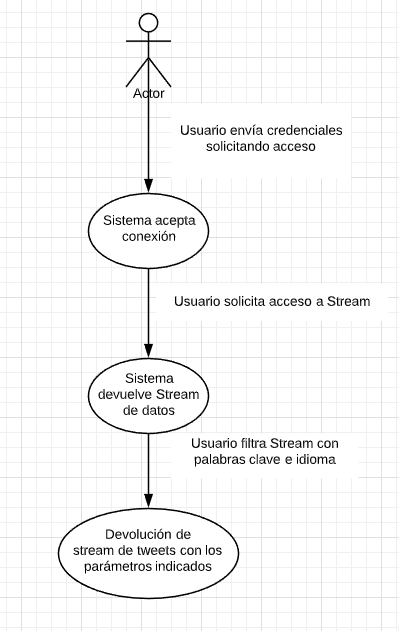
\includegraphics[scale=.4]{imagenes/casoUso1.png}
	\caption{Casos de Uso: Conexión a la API de Twitter.}
	\label{fig:casoUso1}
\end{figure}

\textbf{Conexión a la API de MeaningCloud:}
\begin{itemize}
	\item El usuario solicita conectarse a la API enviando sus credenciales y el texto a analizar
	\item El sistema comprueba las credenciales y analiza el texto. 
	\item El sistema devuelve el resultado del análisis. 
	\item El usuario gestiona los resultados del análisis. 
	\item Si el análisis es exitoso, almacenar los resultados.  
\end{itemize}

\begin{figure}[H]
	\centering
	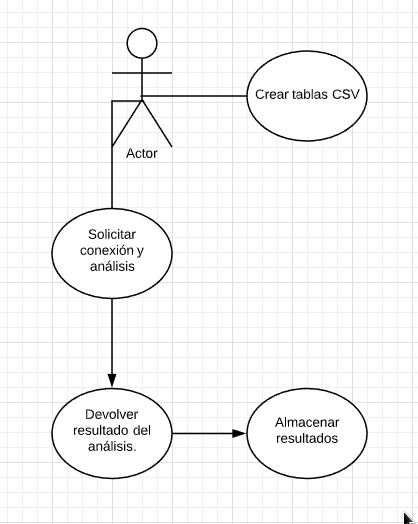
\includegraphics[scale=.4]{imagenes/casoUso2.png}
	\caption{Casos de Uso: Conexión a la API de MeaningCloud.}
	\label{fig:casoUso2}
\end{figure}